%package list
\documentclass{article}
\usepackage[top=3cm, bottom=3cm, outer=3cm, inner=3cm]{geometry}
\usepackage{multicol}
\usepackage{graphicx}
\usepackage{url}
%\usepackage{cite}
\usepackage{hyperref}
\usepackage{array}
%\usepackage{multicol}
\newcolumntype{x}[1]{>{\centering\arraybackslash\hspace{0pt}}p{#1}}
\usepackage{natbib}
\usepackage{pdfpages}
\usepackage{multirow}
\usepackage[normalem]{ulem}
\useunder{\uline}{\ul}{}
\usepackage{svg}
\usepackage{xcolor}
\usepackage{listings}
\lstdefinestyle{ascii-tree}{
    literate={├}{|}1 {─}{--}1 {└}{+}1 
  }
\lstset{basicstyle=\ttfamily,
  showstringspaces=false,
  commentstyle=\color{red},
  keywordstyle=\color{blue}
}
%\usepackage{booktabs}
\usepackage{caption}
\usepackage{subcaption}
\usepackage{float}
\usepackage{array}

\newcolumntype{M}[1]{>{\centering\arraybackslash}m{#1}}
\newcolumntype{N}{@{}m{0pt}@{}}


%%%%%%%%%%%%%%%%%%%%%%%%%%%%%%%%%%%%%%%%%%%%%%%%%%%%%%%%%%%%%%%%%%%%%%%%%%%%
%%%%%%%%%%%%%%%%%%%%%%%%%%%%%%%%%%%%%%%%%%%%%%%%%%%%%%%%%%%%%%%%%%%%%%%%%%%%
\newcommand{\itemEmail}{fayamamani@unsa.edu.pe}
\newcommand{\itemStudent}{Francis Willian Ayamamani Añasco}
\newcommand{\itemCourse}{Programación Web 2}
\newcommand{\itemCourseCode}{1702122}
\newcommand{\itemSemester}{I}
\newcommand{\itemUniversity}{Universidad Nacional de San Agustín de Arequipa}
\newcommand{\itemFaculty}{Facultad de Ingeniería de Producción y Servicios}
\newcommand{\itemDepartment}{Departamento Académico de Ingeniería de Sistemas e Informática}
\newcommand{\itemSchool}{Escuela Profesional de Ingeniería de Sistemas}
\newcommand{\itemAcademic}{2023 - A}
\newcommand{\itemInput}{Del 20 Julio 2023}
\newcommand{\itemOutput}{Al 21 Julio 2023}
\newcommand{\itemPracticeNumber}{07}
\newcommand{\itemTheme}{Django Rest Framework}
%%%%%%%%%%%%%%%%%%%%%%%%%%%%%%%%%%%%%%%%%%%%%%%%%%%%%%%%%%%%%%%%%%%%%%%%%%%%
%%%%%%%%%%%%%%%%%%%%%%%%%%%%%%%%%%%%%%%%%%%%%%%%%%%%%%%%%%%%%%%%%%%%%%%%%%%%

\usepackage[english,spanish]{babel}
\usepackage[utf8]{inputenc}
\AtBeginDocument{\selectlanguage{spanish}}
\renewcommand{\figurename}{Figura}
\renewcommand{\refname}{Referencias}
\renewcommand{\tablename}{Tabla} %esto no funciona cuando se usa babel
\AtBeginDocument{%
	\renewcommand\tablename{Tabla}
}

\usepackage{fancyhdr}
\pagestyle{fancy}
\fancyhf{}
\setlength{\headheight}{30pt}
\renewcommand{\headrulewidth}{1pt}
\renewcommand{\footrulewidth}{1pt}
\fancyhead[L]{\raisebox{-0.2\height}{
\includegraphics[width=3cm]{img/logo_episunsa.png}}}
\fancyhead[C]{\fontsize{7}{7}\selectfont	\itemUniversity \\ \itemFaculty \\ \itemDepartment \\ \itemSchool \\ \textbf{\itemCourse}}
\fancyhead[R]{\raisebox{-0.2\height}{
\includegraphics[width=1.2cm]{img/logo_abet}}}
\fancyfoot[L]{Estudiante Francis Ayamamani Añasco}
\fancyfoot[C]{\itemCourse}
\fancyfoot[R]{Página \thepage}

% para el codigo fuente
\usepackage{listings}
\usepackage{color, colortbl}
\definecolor{dkgreen}{rgb}{0,0.6,0}
\definecolor{gray}{rgb}{0.5,0.5,0.5}
\definecolor{mauve}{rgb}{0.58,0,0.82}
\definecolor{codebackground}{rgb}{0.95, 0.95, 0.92}
\definecolor{tablebackground}{rgb}{0.8, 0, 0}

\lstset{frame=tb,
	language=bash,
	aboveskip=3mm,
	belowskip=3mm,
	showstringspaces=false,
	columns=flexible,
	basicstyle={\small\ttfamily},
	numbers=none,
	numberstyle=\tiny\color{gray},
	keywordstyle=\color{blue},
	commentstyle=\color{dkgreen},
	stringstyle=\color{mauve},
	breaklines=true,
	breakatwhitespace=true,
	tabsize=3,
	backgroundcolor= \color{codebackground},
}

\begin{document}
	
	\vspace*{10px}
	
	\begin{center}	
		\fontsize{17}{17} \textbf{ Informe de Laboratorio \itemPracticeNumber}
	\end{center}
	\centerline{\textbf{\Large Tema: \itemTheme}}
	%\vspace*{0.5cm}	

	\begin{flushright}
		\begin{tabular}{|M{2.5cm}|N|}
			\hline 
			\rowcolor{tablebackground}
			\color{white} \textbf{Nota}  \\
			\hline 
			     \\[30pt]
			\hline 			
		\end{tabular}
	\end{flushright}	

	\begin{table}[H]
		\begin{tabular}{|x{4.7cm}|x{4.8cm}|x{4.8cm}|}
			\hline 
			\rowcolor{tablebackground}
			\color{white} \textbf{Estudiante} & \color{white}\textbf{Escuela}  & \color{white}\textbf{Asignatura}   \\
			\hline 
			{\itemStudent \par \itemEmail} & \itemSchool & {\itemCourse \par Semestre: \itemSemester \par Código: \itemCourseCode}     \\
			\hline 			
		\end{tabular}
	\end{table}		
	
	\begin{table}[H]
		\begin{tabular}{|x{4.7cm}|x{4.8cm}|x{4.8cm}|}
			\hline 
			\rowcolor{tablebackground}
			\color{white}\textbf{Laboratorio} & \color{white}\textbf{Tema}  & \color{white}\textbf{Duración}   \\
			\hline 
			\itemPracticeNumber & \itemTheme & 04 horas   \\
			\hline 
		\end{tabular}
	\end{table}
	
	\begin{table}[H]
		\begin{tabular}{|x{4.7cm}|x{4.8cm}|x{4.8cm}|}
			\hline 
			\rowcolor{tablebackground}
			\color{white}\textbf{Semestre académico} & \color{white}\textbf{Fecha de inicio}  & \color{white}\textbf{Fecha de entrega}   \\
			\hline 
			\itemAcademic & \itemInput &  \itemOutput  \\
			\hline 
		\end{tabular}
	\end{table}
	
	\section{Tarea}
	\begin{itemize}
    \item En sus grupos de trabajo correspondientes. Elabore un servicio web que tenga un CRUD con el uso de este framework.
    \begin{itemize}
        \item Create - POST
        \item Read - GET
        \item Update - PUT
        \item Delete - DELETE
    \end{itemize}
    \item Centrarce en el Core business de su aplicacion web. Los mas importante y necesario que este disponible a traves de un servicio web.
    \item Ejemplos: https://reqbin.com/, https://www.googleapis.com/youtube/v3/playlistItems
    \item Muestre la funcionalidad consumiendola desde el cliente Rest de su preferencia.
    \item El metodo GET puede ser directamente consumido por un navegador web:
    \item Por ejemplo: En esta API se puede obtener la temperatura de Arequipa en un rango de fechas: (La version gratuita tiene un retraso de 7 dıas, por tanto solo mostrara la temperatura en Arequipa desde el 01 de Julio hasta el 03 de Julio)
    \item \url{https://archive-api.open-meteo.com/v1/archive?latitude=-16.39889&longitude=-71.535&start_date=2023-07-01&end_date=2023-07-10&hourly=temperature_2m&daily=temperature_2m_max,temperature_2m_mintimezone=America%2FNew_York}
        \end{itemize}
	\section{MARCO CONCEPTUAL}
	\begin{itemize}
		\item Editor Vim
        \begin{itemize}
            \item Vim es un editor de texto muy eficiente para programar en consola que no tiene nada que envidiar a los editores gráficos.
        \end{itemize}
        \item Instalar Vim en
        \begin{itemize}
            \item GNU/Linux
                \begin{lstlisting}
                    apt-get install vim
                \end{lstlisting}
            \item MS Windows
            \begin{itemize}
                \item Para descarga en sistemas MS Windows \url{https://www.vim.org/download.php}
            \end{itemize}
            \item MacOS
                \begin{lstlisting}
                    brew install macvim
                \end{lstlisting}
        \end{itemize}
        \item Git
        \begin{itemize}
            \item Git es un sistema de control de versiones creado por Linus Torvalds. Es eficiente, confiable.
        \end{itemize}
        \item Instalar Git
        \begin{itemize}
            \item GNU/Linux
                \begin{lstlisting}
                apt-get install git    
                \end{lstlisting}
            \item MS Windows
            \begin{itemize}
                \item Para descarga en sistemas MS Windows \url{https://git-scm.com/download/win}
            \end{itemize}
            \item MacOS
            \begin{itemize}
                \item Para descarga en sistemas MacOS \url{https://git-scm.com/download/mac}
                \begin{lstlisting}
                    brew install git
                \end{lstlisting}
            \end{itemize}
        \end{itemize}
        \item python
        \begin{itemize}
            \item Para un instalación local en sistemas operativos MS Windows utilice: https://www.python.org/downloads/windows/
            \item Tambien ud puede probar código en herramientas online: \url{https://www.programiz.com/python-programming/online-compiler/}
            \item Python en Debian GNU/Linux:
            \begin{lstlisting}[language=bash,caption={Debian Linux viene con Python 3 y Python 2 preinstalados.}][H]
		          python3 --version
                    Python 3.9.2
	        \end{lstlisting}
            \begin{lstlisting}[language=bash,caption={Instalemos pip, una herramienta que instalará y administrará los paquetes de programación que queramos usar en nuestros proyectos de desarrollo.}][H]
		          sudo apt-get install -y python3-pip
	        \end{lstlisting}
            \begin{lstlisting}[language=bash,caption={Paquetes y herramientas de desarrollo más para instalar para garantizar que tengamos una configuración sólida para nuestro entorno de programación:}][H]
		          sudo apt-get install build-essential libssl-dev libffi-dev python3-dev
	        \end{lstlisting}
            \item Configurar un entorno virtual:
            \begin{itemize}
                \item Los entornos virtuales permiten tener un espacio aislado en los proyectos Python
                \item Garantizando que cada proyecto pueda tener su propio conjunto de dependencias que no interrumpirán a otros proyectos.
                \item Manejando diferentes versiones de los paquetes. Esto es especialmente importante cuando se trabaja con paquetes de terceros.
                \item Puede varios entornos de programación.
                \item Cada entorno es un directorio en la que se ubicaran sus scripts.
                \item Usaremos el módulo venv , que es parte de la biblioteca estándar de Python.
                \begin{lstlisting}[language=bash,caption={Entorno de Linux-Instalemos venv escribiendo:}][H]
    		          sudo apt install -y python3-venv
    	        \end{lstlisting}
                \begin{lstlisting}[language=bash,caption={Entorno de Linux-Para crear un ambiente elija en qué directorio.}][H]
    		          mkdir -p ~/unsa/pw2/labs/lab04/entorno
                        cd ~/unsa/pw2/labs/lab04/entorno
    	        \end{lstlisting}
                \begin{lstlisting}[language=bash,caption={Entorno de Linux-En el directorio crea un entorno virtual ejecutando el siguiente comando:}][H]
    		          virtualenv -p python3 .
    	        \end{lstlisting}
                \begin{lstlisting}[language=bash,caption={Entorno de Linux-Ejecute el script de activación para activar el entorno virtual:}][H]
    		          source ../bin/activate
    	        \end{lstlisting}
            \end{itemize}
        \end{itemize}
	\end{itemize}
	
	\section{URL de Repositorio Github}
	\begin{itemize}
		\item URL del Repositorio GitHub para clonar o recuperar.
		\item \url{https://github.com/rescobedoq/pw2/}
		\item URL para el laboratorio 05 en el Repositorio GitHub.
		\item \url{https://drive.google.com/file/d/16wJ-eMwnGHcARjE6_lBICuXEfWS1QelO/view}
	\end{itemize}
	
	\section{Resolucion de la tarea}
    \subsection{Inicio}
    \begin{itemize}
        \item Activar el entorno virtual
        \begin{lstlisting}[language=bash,caption={Entorno de Linux-Ejecute el script de activación para activar el entorno virtual:}][H]
    		          source {{Direccion de tu entorno Virtual}}
    	\end{lstlisting}
         \item Gestionar las versiones instaladas
        \begin{lstlisting}[language=bash,caption={Entorno de Linux-Ejecute el script de activación para activar el entorno virtual:}][H]
    		          pip list
    	\end{lstlisting}
        \item Instalar django
        \begin{lstlisting}[language=bash,caption={Entorno de Linux-Ejecute el script de activación para activar el entorno virtual:}][H]
    		          pip install Django
    	\end{lstlisting}
        \item Verificas
        \begin{lstlisting}[language=bash,caption={Entorno de Linux-Ejecute el script de activación para activar el entorno virtual:}][H]
    		          pip list
                    //resultado:
                        Package    Version
                        ---------- -------
                        asgiref    3.5.2
                        Django     4.0.5 //Variable
                        pip        22.0.4
                        setuptools 62.1.0
                        sqlparse   0.4.2
                        wheel      0.37.1
    	\end{lstlisting}
        \item instalar pillow
        \begin{lstlisting}[language=bash,caption={Entorno de Linux-Ejecute el script de activación para activar el entorno virtual:}][H]
    		          pip install pillow
                    //resultado:
                        Package    Version
                        ---------- -------
                        asgiref    3.5.2
                        Django     4.0.5 //Variable
                        pillow     9.5.0 //variable
                        pip        22.0.4
                        setuptools 62.1.0
                        sqlparse   0.4.2
                        wheel      0.37.1
    	\end{lstlisting}
        \item instalar django-restframework, markdown y django-filter
        \begin{lstlisting}[language=bash,caption={Entorno de Linux-Ejecute el script de activación para activar el entorno virtual:}][H]
                pip install djangorestframework
                pip install markdown
                pip install django-filter                    
                        //resultado:
                        Package    Version
                        ---------- -------
                        asgiref    3.5.2
                        Django     4.0.5 //Variable
                        django-filter 23.2 //Variable
                        djangorestframework 3.14.0 //Variable
                        Markdown 3.4.3 //Variable
                        pillow     9.5.0 //variable
                        pip        22.0.4
                        setuptools 62.1.0
                        sqlparse   0.4.2
                        wheel      0.37.1
    	\end{lstlisting}
        \item Registrando del restframework
        \begin{lstlisting}[language=python,caption={Desarrollo en settings.py}][H]
    		          INSTALLED_APPS = [
                        ...
                        'rest_framework',
                    ]
                    
                    REST_FRAMEWORK = {
                        'DEFAULT_PERMISSION_CLASSES': [
                            'rest_framework.permissions.DjangoModelPermissionsOrAnonReadOnly',
                        ]
                    }
    	\end{lstlisting}
        \item Creaciom de las urls, registrandolos en el restframework
        \begin{lstlisting}[language=python,caption={Desarrollo en la principal urls.py}][H]
    		from rest_framework import routers, serializers, viewsets
            from django.conf import settings
            #importamos los modelos
            from Decoraciones.models import Tipo,Carrito,catalogo,Pedido
            
            class TipoSerializer(serializers.HyperlinkedModelSerializer):
                class Meta:
                    model = Tipo
                    fields = ['Tip']
            
            # ViewSets ...
            class TipoViewSet(viewsets.ModelViewSet):
                queryset = Tipo.objects.all()
                serializer_class = TipoSerializer
            
            class CarritoSerializer(serializers.HyperlinkedModelSerializer):
                class Meta:
                    model = Carrito
                    fields = ['nombre','precio','rutaI']
            
            # ViewSets ...
            class CarritoViewSet(viewsets.ModelViewSet):
                queryset = Carrito.objects.all()
                serializer_class = CarritoSerializer
            
            class CatalogoSerializer(serializers.HyperlinkedModelSerializer):
                class Meta:
                    model = catalogo
                    fields = ['nombre','precio','imagen','tipo']
            
            # ViewSets define the view behavior.
            class CatalogoViewSet(viewsets.ModelViewSet):
                queryset = catalogo.objects.all()
                serializer_class = CatalogoSerializer
            
            class PedidoSerializer(serializers.HyperlinkedModelSerializer):
                class Meta:
                    model = Pedido
                    fields = ['NombreC','telefono','direccion','fecha']
            
            # ViewSets define the view behavior.
            class PedidoViewSet(viewsets.ModelViewSet):
                queryset = Pedido.objects.all()
                serializer_class = PedidoSerializer
            
            router = routers.DefaultRouter()
            router.register(r'Tipo', TipoViewSet)
            router.register(r'Carrito', CarritoViewSet)
            router.register(r'Catalogo', CatalogoViewSet)
            router.register(r'Pedido', PedidoViewSet)
            
            urlpatterns = [
                path('rest/', include(router.urls)),
                path('api-auth/',include('rest_framework.urls', namespace='rest_framework')),
                ...
            ] ...
            
    	\end{lstlisting}
        \item Cada serializador convierte los objetos del modelo en formato JSON y viceversa, y cada conjunto de vistas maneja las solicitudes HTTP para las operaciones CRUD utilizando los métodos HTTP correspondientes (POST, GET, PUT, DELETE). Por ejemplo, el conjunto de vistas "TipoViewSet" maneja las solicitudes HTTP para el modelo "Tipo" utilizando los métodos HTTP POST, GET, PUT y DELETE.
        \item El \textbf{enrutador} de Django REST Framework se utiliza para \textbf{generar automáticamente las URL} para las vistas del conjunto, y se agregan a las URL de la aplicación principal utilizando la función "include". También se agregan otras URL para la autenticación y la administración del sitio.
        \item \textbf{ACLARACION:} La clase producto no puede mostrase, debido a es una plantilla de las base de datos de otros models como carrito, y por ello no es una tabla en la base de datos en si.
        \end{itemize}
    \subsection{Ejecucion}
        \begin{figure}[H]
		          \centering
		          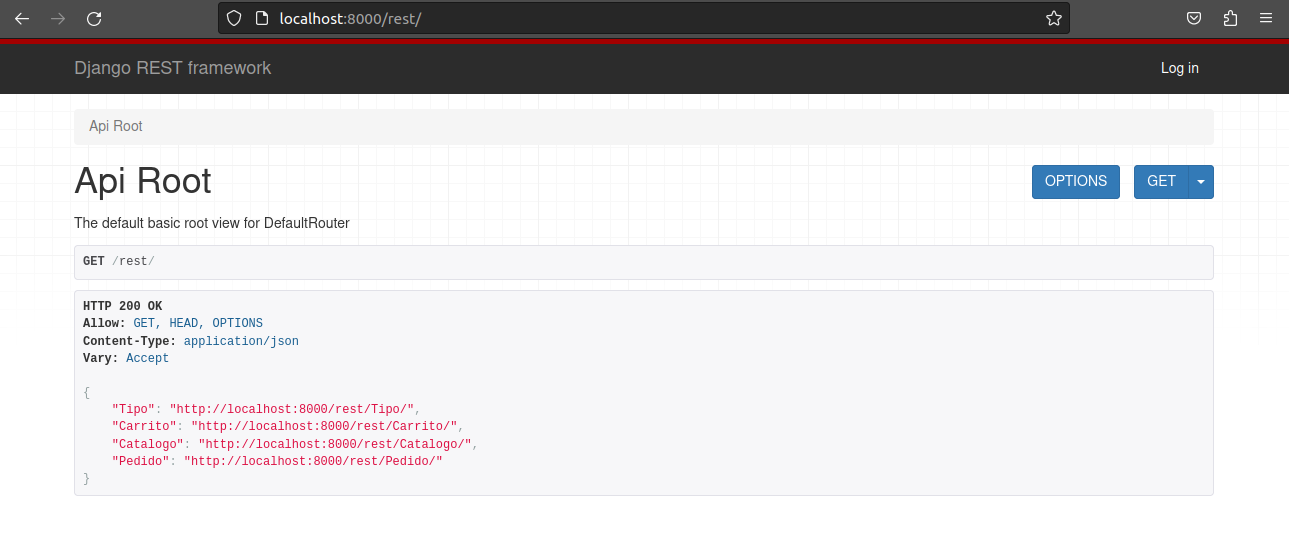
\includegraphics[scale=0.4,keepaspectratio]{img/Captura desde 2023-07-21 08-23-44.png}
		          %\includesvg{img/automata.svg}
		          %\label{img:mot2}
		          %\caption{Product backlog.}
	            \end{figure}
    \begin{itemize}
        \item En este caso se observa la pagina del framework
    \end{itemize}
        \begin{figure}[H]
		          \centering
		          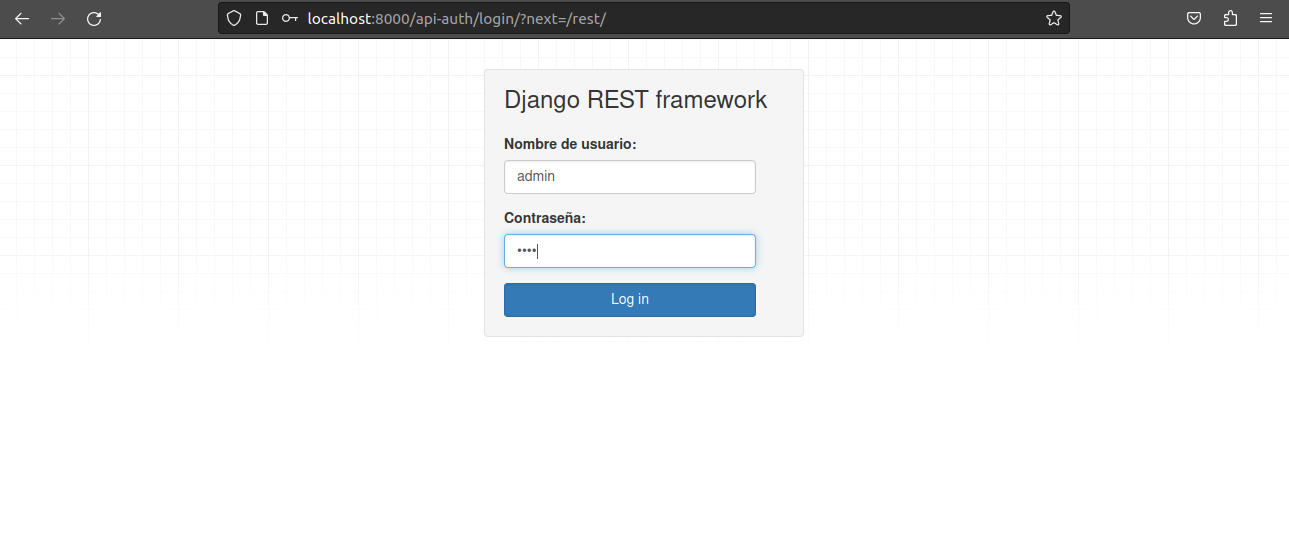
\includegraphics[scale=0.4,keepaspectratio]{img/Captura desde 2023-07-21 08-24-00.png}
		          %\includesvg{img/automata.svg}
		          %\label{img:mot2}
		          %\caption{Product backlog.}
	            \end{figure}
    \begin{itemize}
        \item Vista del login
    \end{itemize}
            \begin{figure}[H]
		          \centering
		          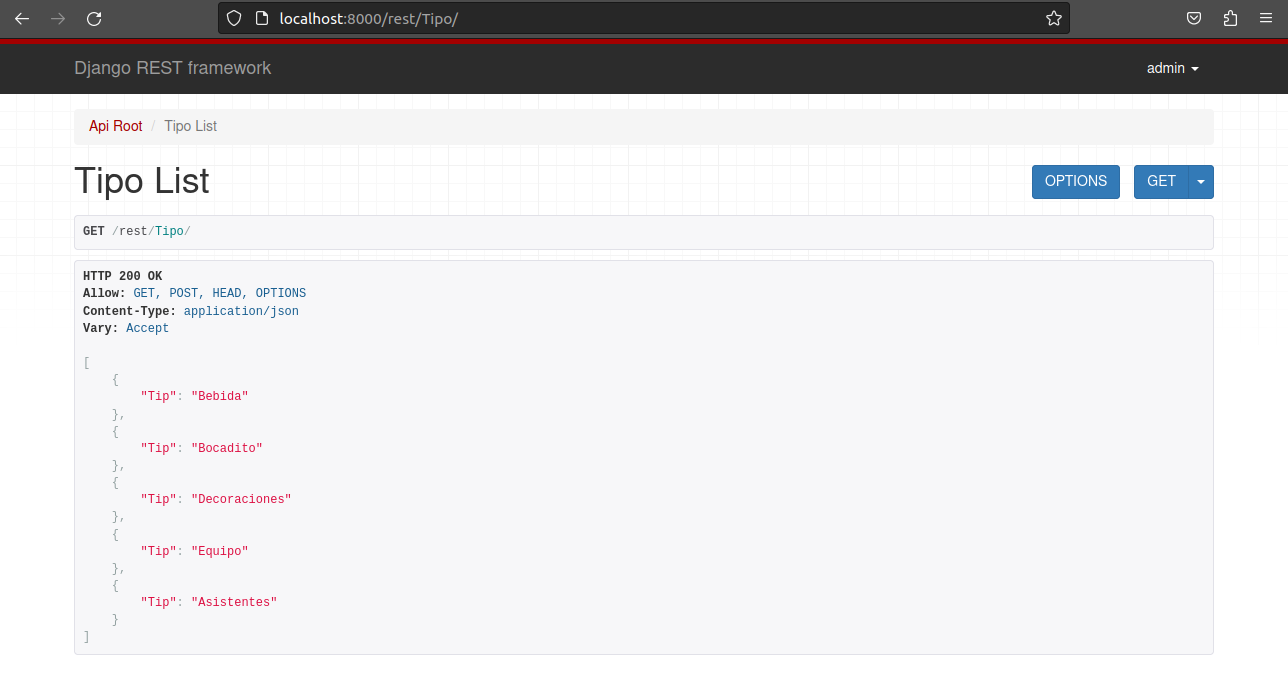
\includegraphics[scale=0.4,keepaspectratio]{img/Captura desde 2023-07-21 08-24-17.png}
		          %\includesvg{img/automata.svg}
		          %\label{img:mot2}
		          %\caption{Product backlog.}
	            \end{figure}
    \begin{itemize}
        \item Vista del model Tipo
    \end{itemize}
    \begin{figure}[H]
		          \centering
		          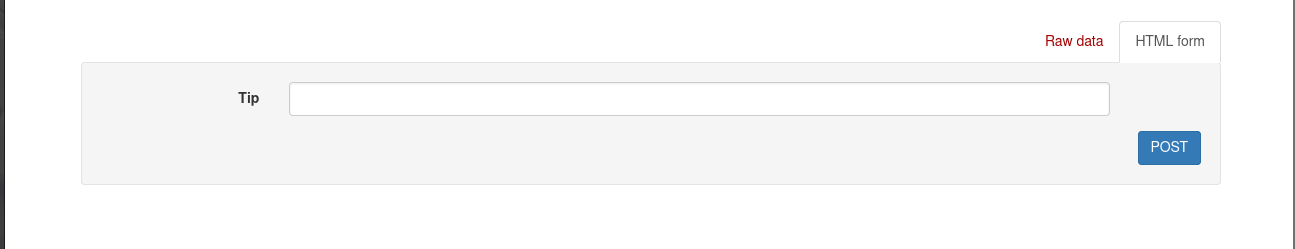
\includegraphics[scale=0.4,keepaspectratio]{img/Captura desde 2023-07-21 08-24-28.png}
		          %\includesvg{img/automata.svg}
		          %\label{img:mot2}
		          %\caption{Product backlog.}
	            \end{figure}
    \begin{itemize}
        \item Vista del PUT
    \end{itemize}
        \begin{figure}[H]
		          \centering
		          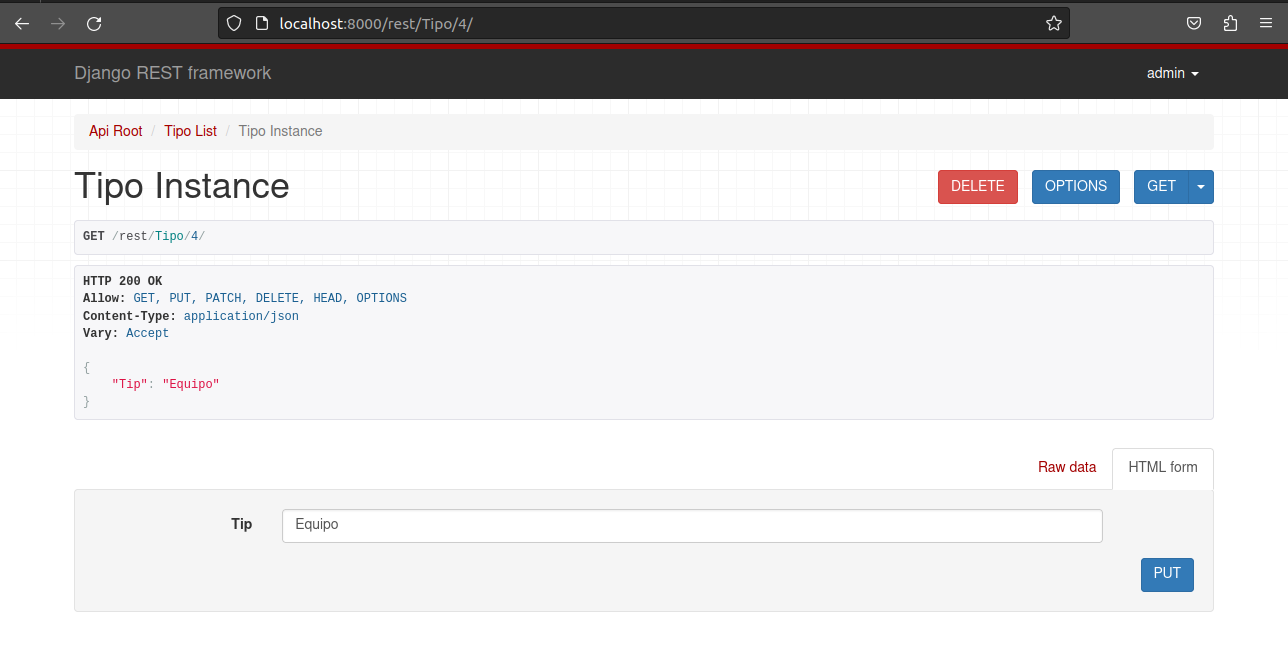
\includegraphics[scale=0.4,keepaspectratio]{img/Captura desde 2023-07-21 08-24-51.png}
		          %\includesvg{img/automata.svg}
		          %\label{img:mot2}
		          %\caption{Product backlog.}
	            \end{figure}
    \begin{itemize}
        \item Vista del Delete, Put, Get; de un objeto.
    \end{itemize}
    \subsection{Commit-GITUHUB}
    \begin{figure}[H]
		          \centering
		          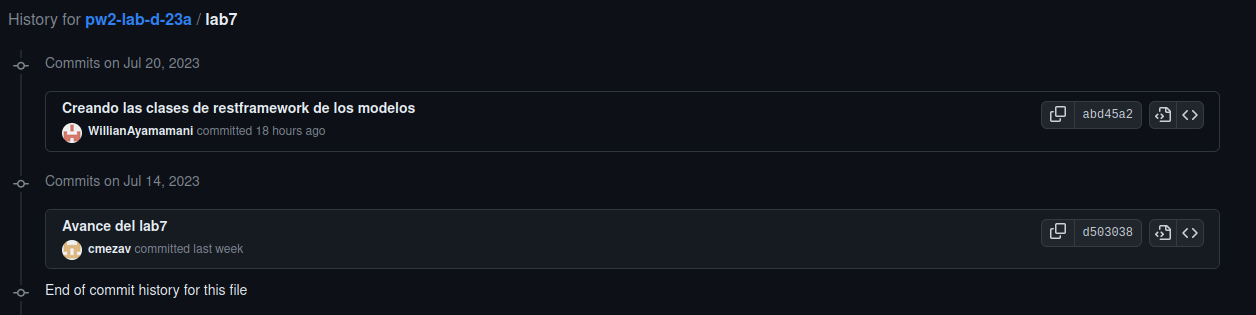
\includegraphics[scale=0.4,keepaspectratio]{img/Captura desde 2023-07-21 09-02-32.png}
		          %\includesvg{img/automata.svg}
		          %\label{img:mot2}
		          %\caption{Product backlog.}
	\end{figure}
    \subsection{USUARIO}
        \begin{lstlisting}[language=bash,caption={Credenciales}][H]
    		          USUARIO:
                        name:usuario1
                        password:Peru1989
                    ADMIN:
                        name:admin
                        password:1234
    	\end{lstlisting}
	\subsection{Estructura de laboratorio 07}
	\begin{itemize}	
		\item El contenido que se entrega en este laboratorio es el siguiente:
	\end{itemize}
\begin{lstlisting}[style=ascii-tree]
lab7/
|--- LATEX/
    |   |--- main.tex
    |   |--- lab7.pdf
    |   |--- img
            |   |--- Captura desde 2023-07-21 08-23-44.png
            |   |--- Captura desde 2023-07-21 08-24-00.png
            |   |--- Captura desde 2023-07-21 08-24-17.png
            |   |--- Captura desde 2023-07-21 08-24-28.png
            |   |--- Captura desde 2023-07-21 08-24-51.png
            |   |--- logo_unsa.jpg
            |   |--- logo_episunsa.png
            |   |--- logo_abet.png
|-- PWB/
        |--- manage.py
        |--- db.sqlite3
        #nombre de mi APP
        |--- Decoraciones/
            |   |--- media/
                |   |--- img/
                    |   |--- Agua.jpg
                    |   |--- Champ.jpg
                    |   |--- concert-2119610_1280.jpg
                    |   |--- D1.jpg
                    |   |--- D2.jpg
                    |   |--- EA.jpg
                    |   |--- EB.jpg
                    |   |--- EC.jpg
                    |   |--- entrada.jpg
                    |   |--- Fondo.jpg
                    |   |--- Juguero.jpg
                    |   |--- Pera.jpg
                    |   |--- Sopero.jpg
                    |   |--- Vino.jpg
            |   |--- static/
                |   |--- Decoracions/
                    |   |--- js
                        |   |--- media/
                    |   |--- style/
                        |   |--- fondo.jpg
                        |   |--- logo.jpg
                        |   |--- nombre.jpg
                        |   |--- nu.jpg
                        |   |--- pr.jpg
                        |   |--- style.css
            |   |--- __init__.py
            |   |--- admin.py
            |   |--- apps.py
            |   |--- models.py
            |   |--- tests.py
            |   |--- views.py
            |   |--- urls.py
        |--- Usuario/
            |   |--- __init__.py
            |   |--- admin.py
            |   |--- apps.py
            |   |--- models.py
            |   |--- tests.py
            |   |--- views.py
            |   |--- urls.py
        |--- PWB/
            |   |--- __init__.py
            |   |--- asgi.py
            |   |--- settings.py
            |   |--- urls.py
\end{lstlisting}    

\section{Cuestionario}
	\begin{itemize}
		\item ¿Cual fue la mayor dificultad del uso de este framework?.
        \\La sintaxis de las importaciones y acceso a las apps.
	\end{itemize}		

	\section{\textcolor{red}{Rúbricas}}
	
	\subsection{\textcolor{red}{Entregable Informe}}
	\begin{table}[H]
		\caption{Tipo de Informe}
		\setlength{\tabcolsep}{0.5em} % for the horizontal padding
		{\renewcommand{\arraystretch}{1.5}% for the vertical padding
		\begin{tabular}{|p{3cm}|p{12cm}|}
			\hline
			\multicolumn{2}{|c|}{\textbf{\textcolor{red}{Informe}}}  \\
			\hline 
			\textbf{\textcolor{red}{Latex}} & \textcolor{blue}{El informe está en formato PDF desde Latex,  con un formato limpio (buena presentación) y facil de leer.}   \\ 
			\hline 
			
			
		\end{tabular}
	}
	\end{table}
	
	\clearpage
	
	\subsection{\textcolor{red}{Rúbrica para el contenido del Informe y demostración}}
	\begin{itemize}			
		\item El alumno debe marcar o dejar en blanco en celdas de la columna \textbf{Checklist} si cumplio con el ítem correspondiente.
		\item Si un alumno supera la fecha de entrega,  su calificación será sobre la nota mínima aprobada, siempre y cuando cumpla con todos lo items.
		\item El alumno debe autocalificarse en la columna \textbf{Estudiante} de acuerdo a la siguiente tabla:
	
		\begin{table}[ht]
			\caption{Niveles de desempeño}
			\begin{center}
			\begin{tabular}{ccccc}
    			\hline
    			 & \multicolumn{4}{c}{Nivel}\\
    			\cline{1-5}
    			\textbf{Puntos} & Insatisfactorio 25\%& En Proceso 50\% & Satisfactorio 75\% & Sobresaliente 100\%\\
    			\textbf{2.0}&0.5&1.0&1.5&2.0\\
    			\textbf{4.0}&1.0&2.0&3.0&4.0\\
    		\hline
			\end{tabular}
		\end{center}
	\end{table}	
	
	\end{itemize}
	
	\begin{table}[H]
		\caption{Rúbrica para contenido del Informe y demostración}
		\setlength{\tabcolsep}{0.5em} % for the horizontal padding
		{\renewcommand{\arraystretch}{1.5}% for the vertical padding
		%\begin{center}
		\begin{tabular}{|p{2.7cm}|p{7cm}|x{1.3cm}|p{1.2cm}|p{1.5cm}|p{1.1cm}|}
			\hline
    		\multicolumn{2}{|c|}{Contenido y demostración} & Puntos & Checklist & Estudiante & Profesor\\
			\hline
			\textbf{1. GitHub} & Hay enlace URL activo del directorio para el  laboratorio hacia su repositorio GitHub con código fuente terminado y fácil de revisar. &2 &X &2 & \\ 
			\hline
			\textbf{2. Commits} &  Hay capturas de pantalla de los commits más importantes con sus explicaciones detalladas. (El profesor puede preguntar para refrendar calificación). &4 &X &2 & \\ 
			\hline 
			\textbf{3. Código fuente} &  Hay porciones de código fuente importantes con numeración y explicaciones detalladas de sus funciones. &2 &X &1 & \\ 
			\hline 
			\textbf{4. Ejecución} & Se incluyen ejecuciones/pruebas del código fuente  explicadas gradualmente. &2 &X &1 & \\ 
			\hline			
			\textbf{5. Pregunta} & Se responde con completitud a la pregunta formulada en la tarea.  (El profesor puede preguntar para refrendar calificación).  &2 &X &2 & \\ 
			\hline	
			\textbf{6. Fechas} & Las fechas de modificación del código fuente estan dentro de los plazos de fecha de entrega establecidos. &2 &X &1 & \\ 
			\hline 
			\textbf{7. Ortografía} & El documento no muestra errores ortográficos. &2 &X &2 & \\ 
			\hline 
			\textbf{8. Madurez} & El Informe muestra de manera general una evolución de la madurez del código fuente,  explicaciones puntuales pero precisas y un acabado impecable.   (El profesor puede preguntar para refrendar calificación).  &4 &X &1 & \\ 
			\hline
			\multicolumn{2}{|c|}{\textbf{Total}} &20 & &12 & \\ 
			\hline
		\end{tabular}
		%\end{center}
		%\label{tab:multicol}
		}
	\end{table}
	
\clearpage

\section{Referencias}
\begin{itemize}			
    \item \url{https://github.com/WillianAyamamani/pw2-lab-d-23a/tree/main/lab7}
\end{itemize}	
	
%\clearpage
%\bibliographystyle{apalike}
%\bibliographystyle{IEEEtranN}
%\bibliography{bibliography}
			
\end{document}